\documentclass[a4paper]{report}

\usepackage{amsmath}
\usepackage{amssymb}
\usepackage{graphicx}
\usepackage{textcomp}
%\usepackage{indentfirst}
\usepackage{titlesec}
\usepackage{fancyhdr}
\usepackage[backend=bibtex, style=ieee]{biblatex}
\usepackage{verbatim}
\usepackage[a4paper, margin=2cm]{geometry}
\usepackage{listings}
\usepackage{float}

\addbibresource{bib.bib}

\lstset{
  basicstyle=\ttfamily,
  columns=fullflexible,
  keepspaces=true,
}

\title{
\large{Computer Science and Engineering Department, Chinese University of Hong Kong}\\
~\\
\huge{Code Block Online IDE\\
Final Report}\\
~\\
\large{CSCI3100 Group 18}\\
~\\
\large{Document Version 1.0}\\
}
\author{
CHEUNG Ka Wai\\
SID:1155110140
\and
FENG Haolin\\
SID:1155110663
\and
LEE Tsz Yan\\
SID:1155110177
\and
YU Chi To\\
SID:1155110447}

\titleformat{\chapter}[display]
{\bfseries\Large}
{\thechapter}
{1ex}
{\titlerule\vspace{1ex}\filleft}
[\vspace{1ex}\titlerule]

\pagestyle{fancy}
\fancyhead[L]{Code Block Online IDE}
\fancyhead[R]{\leftmark}

\setlength\parindent{0pt}

\renewcommand{\chaptermark}[1]{\markboth{\MakeUppercase{\thechapter.\ #1}}{}}

\begin{document}
  \pagenumbering{gobble}
  \maketitle
  \tableofcontents
  \newpage
  \pagenumbering{arabic}

  \chapter{Introduction}
\section{Project Overview}
The Code Block Online IDE provides a place for programmers to test and share their code. It is a platform for programmers to share their knowledge on coding and learn from each others on the forum. Programmers can also prototype their code on this online IDE to test out their codes, and share it with the others.

\section{Objective}
Programming skills has become more and more inportant throughout the world. And the promotion of STEM education is now worldwide and implemented in large scale. However, while the traditional text-based coding may be efficient, but they may not be able to arouse the attention to younger kids. While there are some visualised coding platforms available, but they are not well designed for older kids to ask and discuss on a problem.

~

Therefore, the Code Block Online IDE is designed to adapt to the problem. Beginners in programming can learn coding using the visualised online C programming IDE. For advanced programmers, they can simply type in the textbox for higher efficiency. And they can share their code for discussions or questions using the forum. We hope that this kind of forum design, that each post must be connected to a program will help creating a platform like quora, but aimed at programming, where people can exchange their thoughts on their codes.

~

The IDE designed may also be a tool for rapid prototyping. Although there is a current limitation on storing the visualised code, which hindered its usage on rapid prototyping, and there is not enough libraries pre-written for prototyping. But it can still be used for the purpose by drag-and-drop functions built into suitable locations thus may help when prototyping programs.

\section{Highlights}
\subsection{Visualised Code Editor}
The visualised code editor is one of the core highlights of the Code Block Online IDE. The visualised code editor allows beginners in programming to have a more vivid understanding on the meaning of each component of their program. Users of the editor drag suitable blocks of code into the coding area. And the corresponding code will be generated immediatly below the drag-and-drop area so that they can have an overview on the program written. Authenticated users can then choose to save the code on our platform and run it on our server or choose to copy it down and run on their local computer.

\subsection{Forum}
We encourage every user to share and discuss their knowledge. The forum allows authenticated users to share their code and discuss about it here. Each post must have a source code attached with it to act as an example for efficient discussion. Users can post their code and the problem they faced here, so that other users can answer and explain the problem directly and easily. Users can also share their experiences with their code here to the others. And other users interested in the topic can discuss and use the code shared to their expense. For unauthenticated guest users, they can still browse the posts in the forum to gain knowledge here.

\subsection{Server-based Code Compilation and Execution}
Like many other online program compilation and execution websites, the source code is compiled and executed at the server. This is to prevent posing security threats to client's computer by allowing an unknown excutable running on their computer. Another reason for server-based code compilation and execution, is for the ease of coding assignment verification. In programming courses, one of the biggest problemed faced by the students is the difference in output when the output of their assignment is compared with that of the standard answer's. And that is the portability problem. Server-based compilation for both standard answer from teachers and assignment hand-ins from students will solve the problem as their code will be ran on the same operating system. Therefore the protability problem is solved.

\subsection{Search Engine}
In order for efficient knowledge exchange between users, we must ensure users can find the materials they need. Therefore we provide search to all users so that they can find posts that contain the information they need. We allow users to use username, words in title, words in post content and words in reply content as search kwyword. Users can type in any keyword in the search field. The server will find the keyword in all posts for result. This way, users can have an easy access to knowledge they need.

\subsection{Personal Account System}
As we expected educational institutions to use this platform for teaching, we have classified accounts into 3 types. First, normal user accounts that are not related to any educational institutions. Second, user account for teachers, and third, student user accounts. For teacher accounts, they can check coding assignments of students using teacher accounts. They can also find out what posts their students have posted so that they can know the difficulties of students faced when studying this course. For student accounts, users of this type of accounts will can find out the posts of their teacher easily as they are also listed on their user page. Therefore, teachers can use this platform to understand the need of students by checking on the posts posted by students on different problems or as a respond on the material posted on posts by lecturers here., and release assignments or extra materials here to their student.

\newpage

\section{Project Statistics}
ES6-Plato is used to generate the statistics for server and website Javascripts\cite{ES6-Plato}.

\begin{tabular}{|l|l|l|}
  \hline
  File Name & SLOC & McCabe's Number\\
  \hline\hline
  \multicolumn{3}{l}{Server Node.js Scripts}\\
  \hline\hline
  app.js & 811 & 89\\
  \hline
  code.js & 115 & 7\\
  \hline
  compAndRun.js & 101 & 10\\
  \hline
  connect\_sql.js & 980 & 94\\
  \hline
  forum.js & 140 & 5\\
  \hline
  php\_parser & 44 & 2\\
  \hline
  user.js & 100 & 4\\
  \hline\hline
  \multicolumn{3}{l}{Webpage Javascripts}\\
  \hline\hline
  code\_result.js & 14 & 1\\
  \hline
  deletePost.js & 20 & 6\\
  \hline
  redir.js & 5 & 1\\
  \hline
  submitUser.js & 121 & 20\\
  \hline
  submitForm.js & 29 & 6\\
  \hline\hline
  \multicolumn{3}{l}{EJS-Written Website Templates}\\
  \hline\hline
  account\_header.ejs & 10 & 1\\
  \hline
  change\_password.ejs & 11 & 1\\
  \hline
  code\_result.ejs & 24 & 1\\
  \hline
  code.ejs & 24 & 1\\
  \hline
  create\_account.ejs & 33 & 1\\
  \hline
  forum\_header.ejs & 12 & 1\\
  \hline
  forum\_search.ejs & 21 & 3\\
  \hline
  forum.ejs & 25 & 3\\
  \hline
  login.ejs & 32 & 1\\
  \hline
  mainpage.ejs & 36 & 1\\
  \hline
  navbar.ejs & 51 & 3\\
  \hline
  new\_post.ejs & 38 & 2\\
  \hline
  post.ejs & 39 & 3\\
  \hline
  search.ejs & 16 & 1\\
  \hline
  student\_profile.ejs & 33 & 4\\
  \hline
  student.ejs & 53 & 7\\
  \hline
  teacher.ejs & 53 & 7\\
  \hline
  user\_profile.ejs & 28 & 3\\
  \hline
  user.ejs & 46 & 5 \\
  \hline
  Workspace.ejs & 231 & 1\\
  \hline
\end{tabular}

  \chapter{System Architectural Design by DFD}
\section{Architectural Diagram}
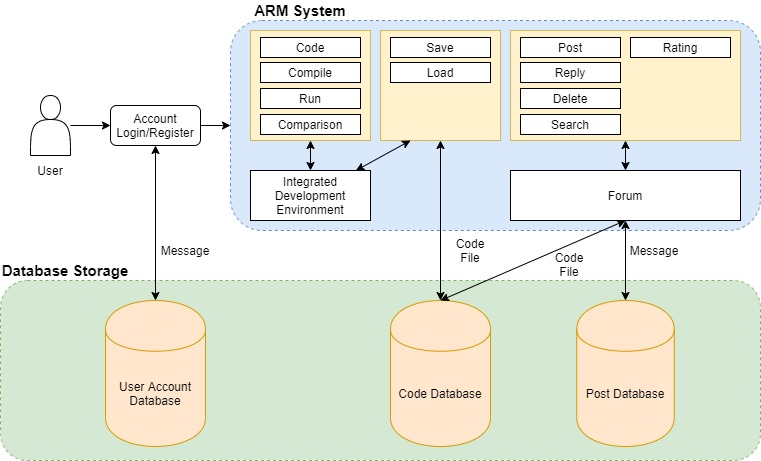
\includegraphics[scale=0.5]{Doc/Pics/architectural_diagram}
\newpage
\section{System Components}
\begin{enumerate}
	\item Personal Account System: Users Information are stored into the user database. Based on current design, users are classified into 3 class, normal user, student and teacher. They have no differences in this phase.
	\item Forum System: Posts are stored into the post database. List of post threads created by users, allows users to post and comment with thier source code. Users' posts can be searched and display to other users.
	\item Code Running System: Source code are stored into the code database. Source code created by users can be compiled, saved and load. Compiled program can be executed and its output will be shown.
\end{enumerate}
\section{Database}
\begin{enumerate}
	\item User Account Database includes username, account password, account type, extra permission of the account for teachers and student users to access posts only available to the class.
	\item Post Database includes posts contents (contents, author, reply, source code linkage, permission) and access frequencies of posts.
  \item Code Database includes source code file, author of the code, filename.
\end{enumerate}
\section{Data Flow Diagram(DFD)}
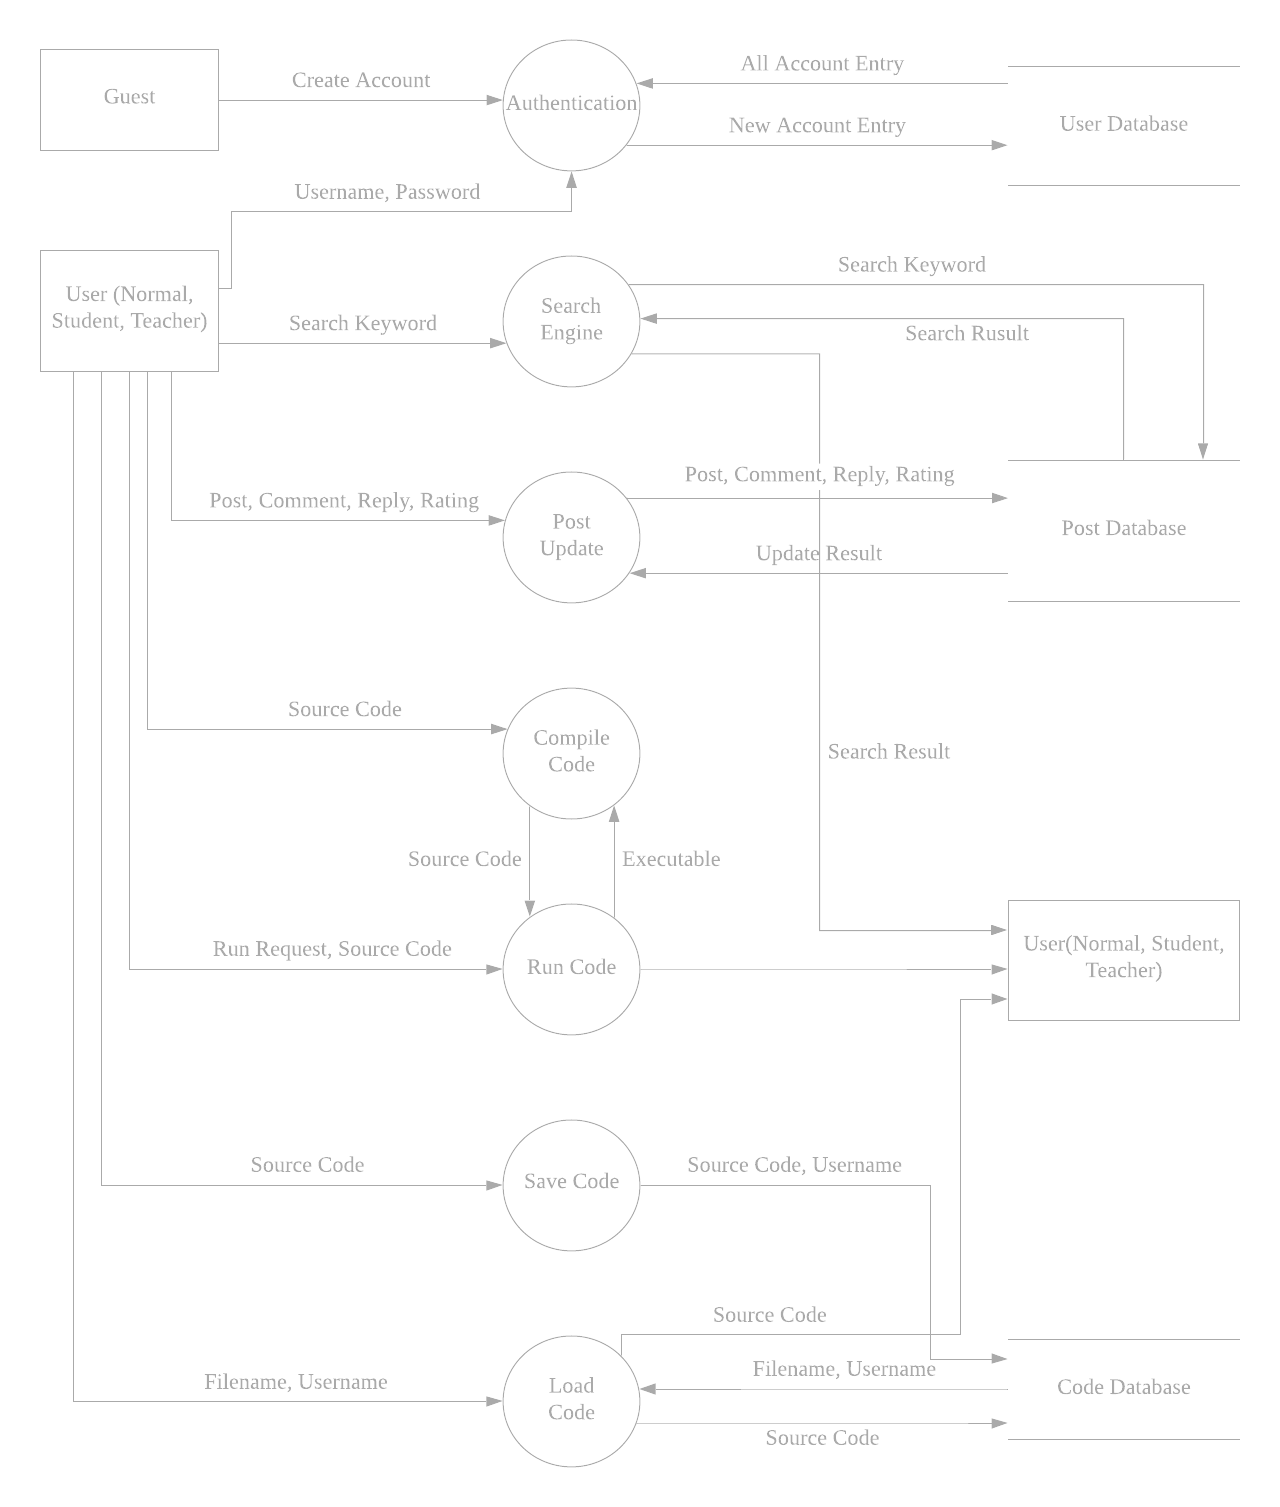
\includegraphics[scale=0.35]{Doc/Pics/dataflow_diagram}

  \clearpage
\section{General Class Diagram}
The following UML Diagram shows all the classes and relationships in the whole system.\newline
The main class server uses three classes which are User, Code and Forum class. User class uses USER class, Forum class uses POST class and Code class uses compAndRun and SRC\_CODE class. USER, POST and SRC\_CODE classes are extended from MySQLDatabase class\newline
\begin{figure}[H]
 \center{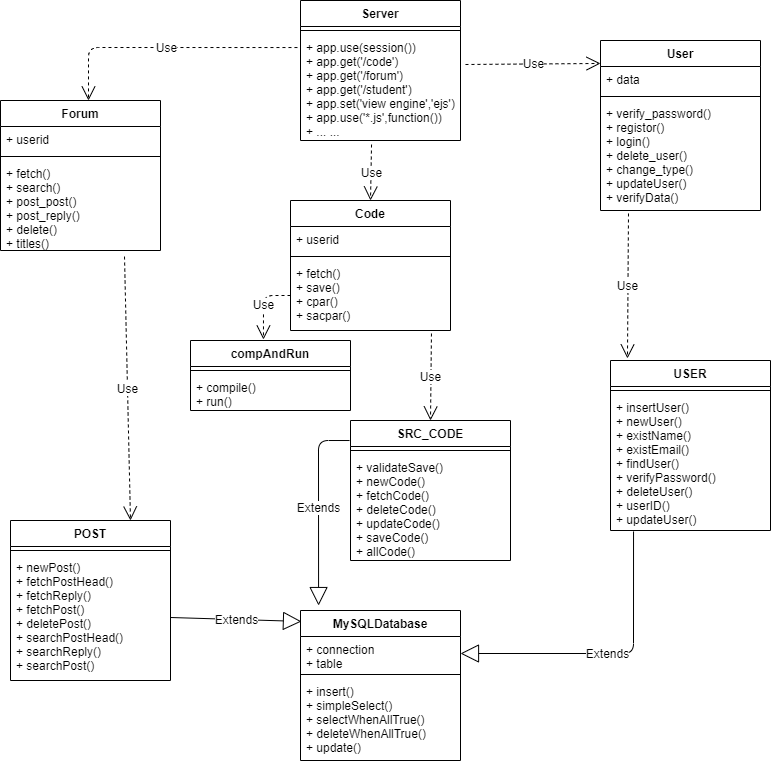
\includegraphics[width=\textwidth]  {Pics/general_class.png}} 
 \label{1}
 \end{figure}
\clearpage

\section{Component-1: Personal Account System}
Personal Account System is a database to provide the identity for student user or teacher user in server and provide several functionalities to user.\newline

\subsection{Use Case Diagram}
\begin{figure}[H]
 \center{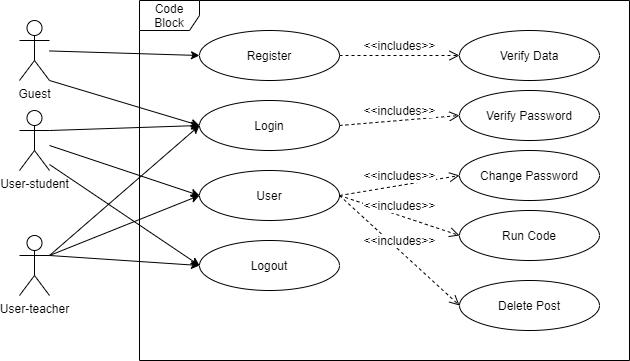
\includegraphics[width=\textwidth]  {Pics/account_use-case.png}}
 \label{2}
 \end{figure}
For a new coming guest, Personal Account System allows he/she can either go to register or login. The register function includes verify data function to verify whether the guest's inputs are all validated. The login function includes verify password function to verify the password input by guest by finding in the database.\newline
For student and teacher user, Personal Account System allows he/she to login and view his/her profile page. The user function provides a page for user to change his/her password, run his/her code and delete his/her post.\newline

\subsection{Sequence Diagram for Guest}
\begin{figure}[H]
 \center{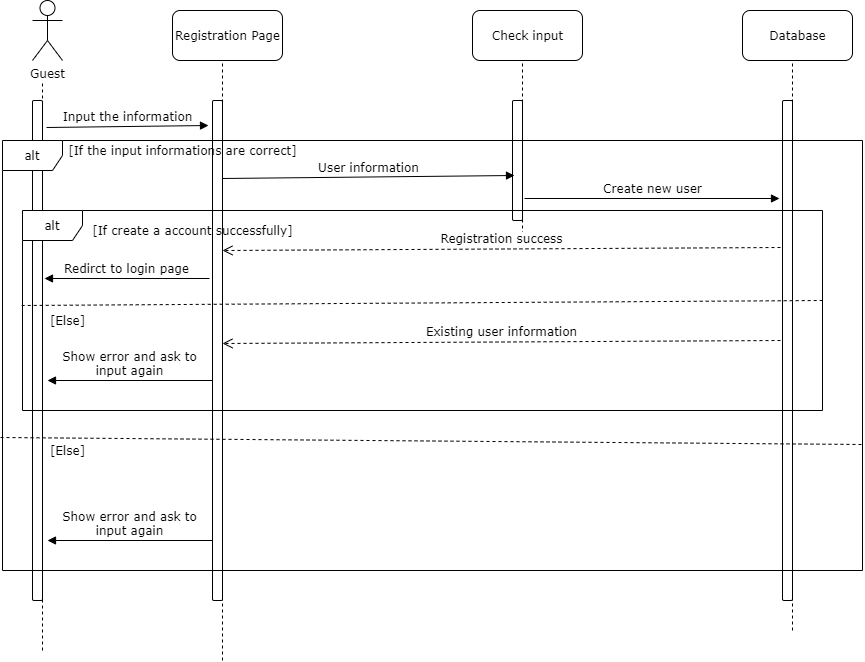
\includegraphics[width=\textwidth]  {Pics/account_sequence_guest.png}} 
 \label{3}
 \end{figure}

\subsection{Activity Diagram for Guest}
\begin{figure}[H]
 \center{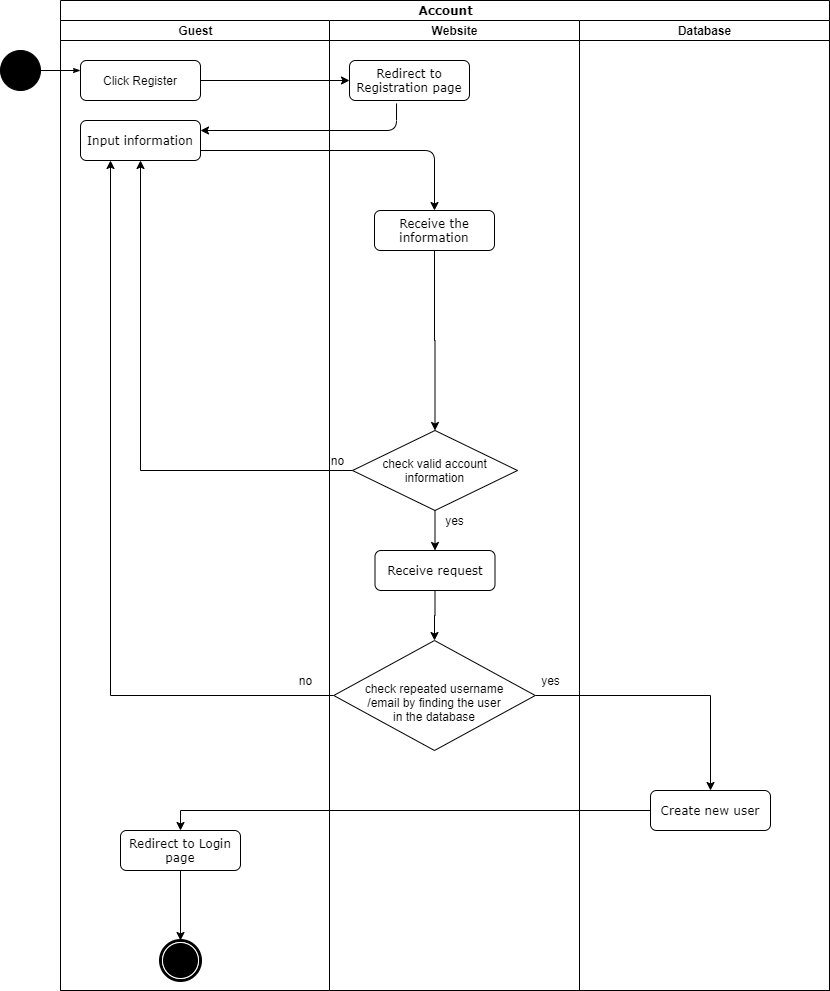
\includegraphics[width=\textwidth]  {Pics/account_activity_guest.png}} 
 \label{4}
 \end{figure}

\subsection{Sequence Diagram for User(login and change password for both types of user)}
\begin{figure}[H]
 \center{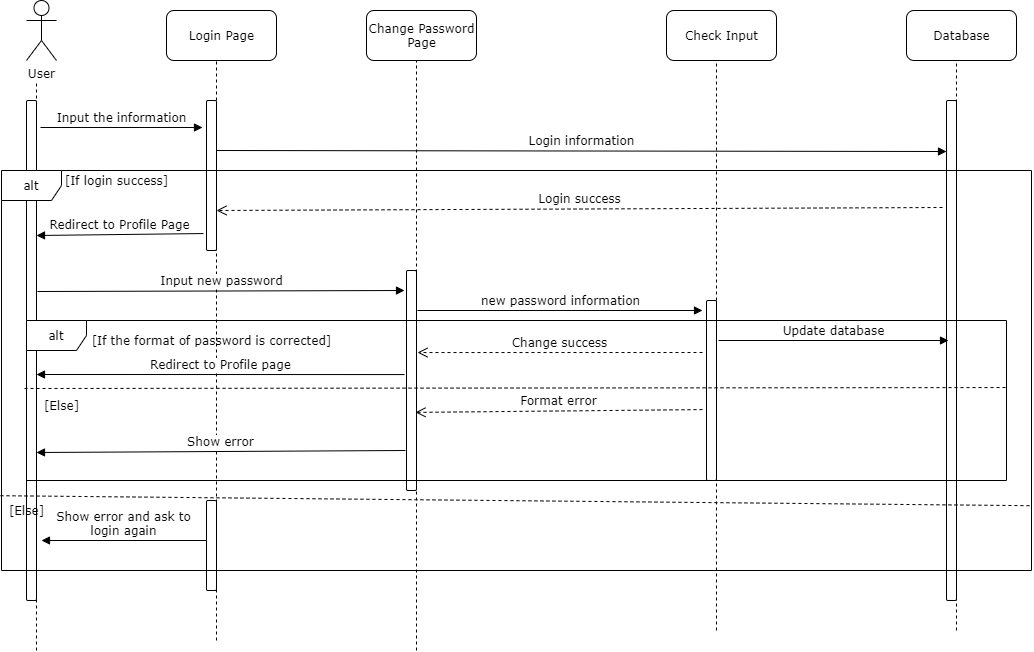
\includegraphics[width=\textwidth]  {Pics/account_sequence_user.png}} 
 \label{10}
 \end{figure}

\subsection{Activity Diagram for User(login and change password for both types of user)}
\begin{figure}[H]
 \center{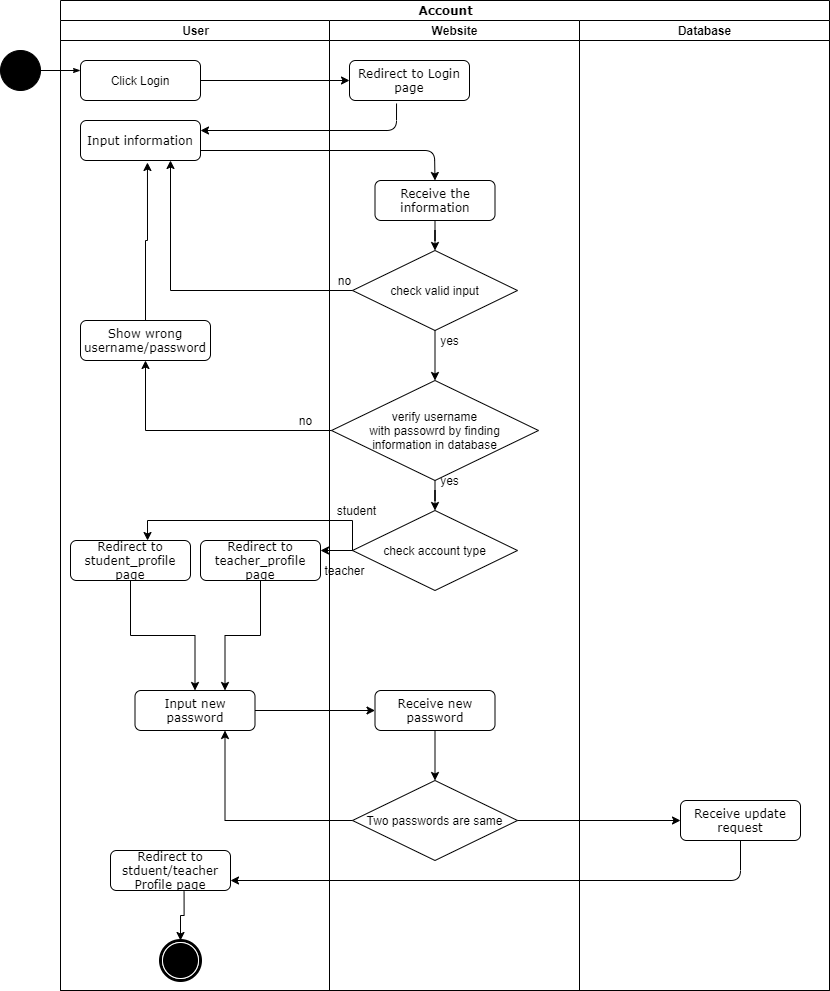
\includegraphics[width=\textwidth]  {Pics/account_activity_user.png}} 
 \label{5}
 \end{figure}

\subsection{Functionality}
This component provided user authentication. It prevented guest without authentication to use some functions which need user identity. For example, writing code, new post and reply. It also provides an easier way for the system to record all the codes, posts and replies that created by that person and user can retrieve those information.\newline

\subsection{Procedures and Functions}
This component provides front-webpages, which are registration page, login page and profile page.\newline\newline
The registration and login page provide basic input checking(format, completion, and length) before passing data request to the server side. After passing the input checking, the webpages will send requests to the database, verifying the data, whether the guest input available username and verifying the password correctness, whether the use login with correct pair of username and password.\newline\newline
The profile page allows users to change their password, run their code and delete their posts. In this page, users can find their profile with username, codes and posts. This page will send a request to server side, getting those information. When user wants to change password, it will do the password verifying for user input, then it will send the request to the server side, changing the password.\newline\newline
For the backend application part, there are lots of functions with SQL statement to retrieve data or update data from the database. It will return the result to the front-webpages after retrieving or updating data, whether it is successful to get or update data.\newline\newline
In conclusion, this system contains the following functions:\newline

\begin{itemize}

\item
\textbf{Registration}
, which is for the guest to register account. This function will verify the data that guest inputs is valid. If the data is valid, create a new account related to the data provided by the guest and redirect to the login page, otherwise, request the guest to input data in correct format.\newline

\item
\textbf{Login}
, which gets the username and password input by user, then verify the correctness from the database. If the input is valid, login to the server, otherwise request the user to input again.\newline

\item
\textbf{Change password}
, which gets the two passwords input by user, then verify whether the two inputs are the same. If the inputs are valid, request server to update the information in database, otherwise request the user to input again.\newline

\item
\textbf{Run code}
, which allow user to choose one of his/her code and redirect to that code page for user to run.

\item
\textbf{Delete Post}
, which allow user to delete the posts wrote by him/her.

\item
\textbf{Logout}
, which stops the access permission with a logged in account.

\end{itemize}
\clearpage

\section{Component-2: Forum}
This is a forum like a system for users to show their codes and discuss on them. The user can write new post, reply to the post, view post and search post.\newline

\subsection{Use Case Diagram}
\begin{figure}[H]
 \center{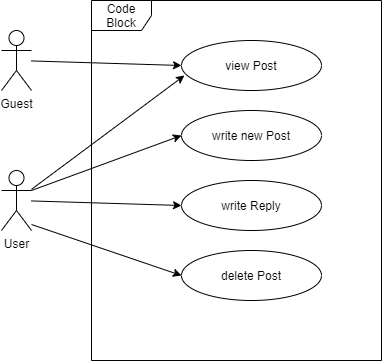
\includegraphics[width=\textwidth]  {Pics/forum_use-case.png}} 
 \label{6}
 \end{figure}
In this system, functions are limited to a guest, guest can only view post and search post. A user is allowed to write new post and write reply. The new post function includes load user code function to list out all the codes that user wrote by finding in the database.\newline

\subsection{Sequence Diagram for Writing new Post and Reply}
\begin{figure}[H]
 \center{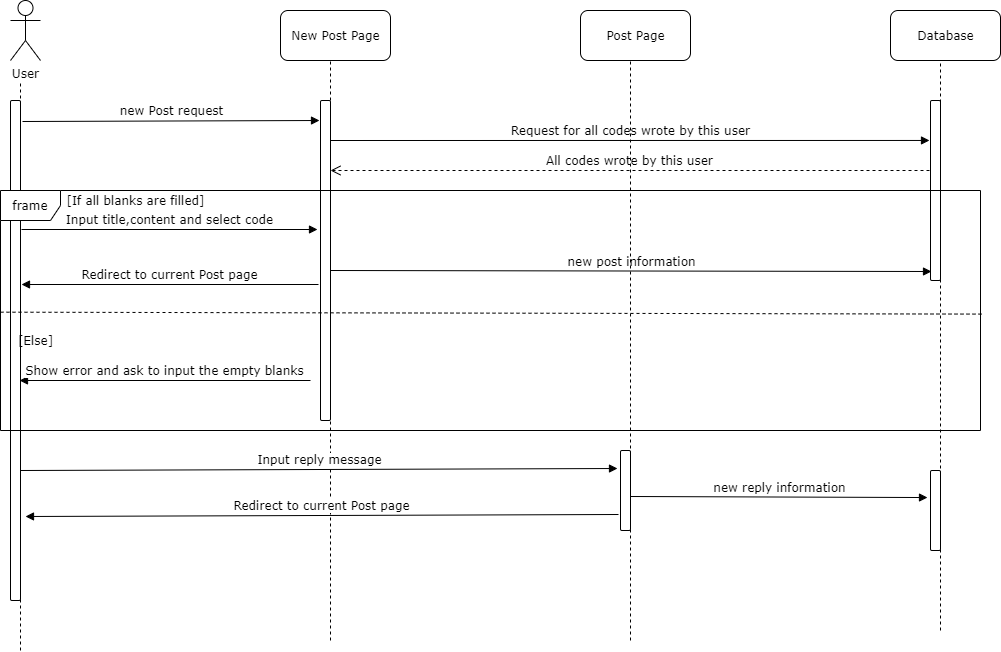
\includegraphics[width=\textwidth]  {Pics/forum_sequence.png}} 
 \label{7}
 \end{figure}

\subsection{Functionality}
The forum component provides a platform for the user to post their code and discuss with other. It contains search post, view post, write new post, write reply functions. Everyone(guest and user)can view post and search post. Only users are allowed to write new post and write reply. If user wants to write a new post but he/she doesn't input title, content and select a code, the page will request user to input all the information, otherwise request the server to update a new post in database.\newline

\subsection{Procedures and Functions}
For the front-end part, the system provided view forum, view post, search post and write new post these 3 pages. For guest, the system will only display view post without reply function, view forum and search post.\newline\newline
In view forum,view post and search post, guests and users are allowed to click inside, viewing the content. When they enter these pages, the server will receive the searching request, and return the required result.\newline\newline
In addition, users are allowed to write new post with the new post page. Users are required to fill in the title, content and select one of their codes in the page. Then the whole data set will be sent to the database, and the server will redirect user to that post page. In a post page, users are allowed to write reply, and the reply will be saved into the database.\newline\newline
In conclusion, this system contains the following functions:

\begin{itemize}

\item
\textbf{View Post}
, which is for everyone(guest and user) to view the post and reply content.\newline

\item
\textbf{Search Post}
, which is a search function receive keyword input by guest or user and return all matching posts.\newline

\item
\textbf{New Post}
, which is for user to write new post with selecting a code and save into the database.\newline

\item
\textbf{Write Reply}
, which is for user to write reply in the post and save into the database.\newline

\end{itemize}
\clearpage

\section{Component-3: Code}
This is a workplace like a online IDE for users to write code in a simple and visualized system.User can drag the block and drop it on the workplace to do coding. The system will automatically generate the code in text format. The user can also save code and run code.\newline

\subsection{Use Case Diagram}
\begin{figure}[H]
 \center{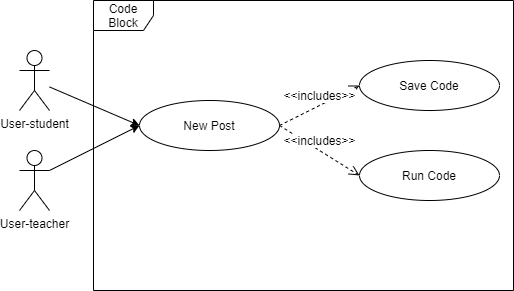
\includegraphics[width=\textwidth]  {Pics/code_use-case.png}} 
 \label{8} 
 \end{figure}
In this system, functions are only provide to user, so guest should register a account first. User is allowed to write code. The write code function includes save code and run code functions.\newline

\subsection{Sequence Diagram for Writing Code, Saving Code and Running Code}
\begin{figure}[H]
 \center{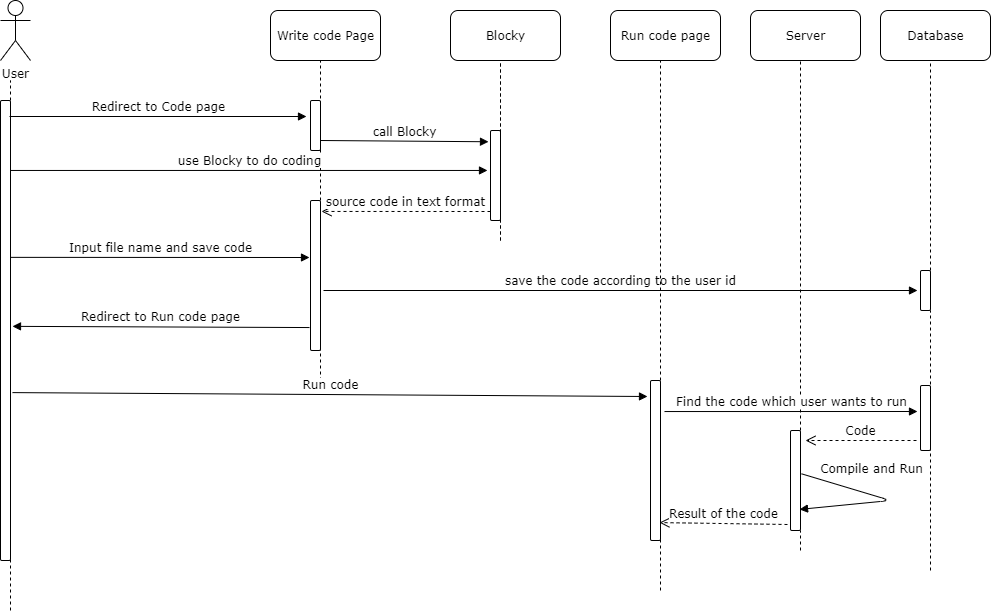
\includegraphics[width=\textwidth]  {Pics/code_sequence.png}} 
 \label{9}
 \end{figure}

\subsection{Functionality}
The code component provides a workplace for the user to do coding online. It contains write code, save code and run code. Only user can use all these functions. 

\subsection{Procedures and Functions}
This component provides front-webpages, which are workplace page, code page and result page.\newline\newline
The workplace page provides a visualized coding area, a code generation area and a form to save code. User should input the file name and copy the code from the code generation area to the form, then the page will send request to server to save the code into the database according to the user identity. After that, the server will redirect the user to that code page.\newline\newline
The code page shows the code wrote by the user for viewing, and there is a input area is used for STDIN when the program required input from keyboard. User can run the code in this page, the page will send the request with the code and input data to server, server will do the compilation and execution. After that, the server will redirect user to result page and return the code result to that page.\newline\newline
For the backend application part, there are lots of functions with SQL statement to retrieve data or update data from the database. Server handles the run code request and return the result to the result page.\newline\newline
In conclusion, this system contains the following functions:\newline

\begin{itemize}

\item
\textbf{Write Code}
, which is for user to do coding in a simple and visualized workplace. User can drag the block and drop it on the workplace and the system generates code in text format.\newline

\item
\textbf{Save Code}
, which is for user to save the code he/she writes. User should input the file name then copy and paste the code generated by the system into the form, then the page sends request to server and ask to update the database according to the user identity. After that, the server redirects user to that code page.

\item
\textbf{Run Code}
, which is for user to run his/her code with optional STDIN input. It sends requests with code and input data to server, server handles the request then do compilation and execution. After that, the server redirects user to result page and return the code result in that page.

\end{itemize}
  \chapter{User Interface Design}

  \chapter{Test}
\section{Overview and Plan}
The system is tested using black-box testing and bottom-up integration test. Black-box testing is used as the functions and modules designed may not act according to our specification. Bottom-up integration test is chosen for the system as the system relies heavily on two slave modules. Thus the correctness of the system relies heavily on the two slave modules. Module inputs and user activities are tested using black-box testing to ensure correctness of the system.

\section{MySQL Database Interface Module}
\subsection{Purpose}
The connect\_sql.js is tested in this testcase to ensure the correctness of this slave module that act as an interface to communicate between the server and the database. All child classes inherits and reuses the methods of parent class MySQLDatabase, therefore only the major functions of parent class is tested using methods of child classes

\subsection{Inputs}
\subsubsection{Insert}
Test cases of USER used (USERNAME, EMAIL, PASSWORD, ACC\_TYPE):
\begin{enumerate}
  \item newUser, newUser@localhost.net, 11111111, 0 (valid)
  \item (empty), no@here, (empty), 0 (invalid empty input)
  \item no, no, no, no (wrong ACC\_TYPE type)
\end{enumerate}

\subsubsection{Select When All Conditions Are True}
Test cases of SRC\_CODE used (NAME, USER):
\begin{enumerate}
  \item hello\_world.c, 1 (valid)
  \item (empty), 1 (empty name)
  \item here, ADMIN (wrong USER type)
\end{enumerate}

\subsubsection{Delete When All Conditions Are True}
Test cases of SRC\_CODE used (NAME, USER)
\begin{enumerate}
  \item hello-world.c, 1 (valid)
  \item (empty), 1 (empty NAME)
  \item here, ADMIN (wrong USER type)
\end{enumerate}

\subsubsection{Update}
Test cases of USER used (PASSWORD, ID):
\begin{enumerate}
  \item 88888888, 10 (valid)
  \item (empty), 10 (empty PASSWORD)
  \item hello\_goodbye, newUser (wrong ID type)
  \item 88888888, 0 (invalid ID)
\end{enumerate}

\subsection{Expected Outputs \& Pass/Fail Criteria}
The testcases demonstrates the return of the module when different input is provided, both valid and invalid queries to the MySQL database. The module should handle the exception and provide error message for unaccepted invalid testcases and return a ``fail'' message, and provide result for accepted valid or invalid testcases.
\subsubsection{Insert}
Case 1:
\verbatiminput{Doc/test/case1-1-1.txt}

Case 2:
\verbatiminput{Doc/test/case1-1-2.txt}

Case 3:
\lstinputlisting[breaklines]{Doc/test/case1-1-3.txt}

\subsubsection{Select When All Conditions Are True}
Case 1:
\lstinputlisting[breaklines]{Doc/test/case1-2-1.txt}

Case 2:
\verbatiminput{Doc/test/case1-2-2.txt}

Case 3:
\verbatiminput{Doc/test/case1-2-3.txt}

\subsubsection{Delete When All Conditions Are True}
Case 1:
\verbatiminput{Doc/test/case1-3-1.txt}

Case 2:
\verbatiminput{Doc/test/case1-3-2.txt}

Case 3;
\verbatiminput{Doc/test/case1-3-3.txt}

\subsubsection{Update}
Case 1:
\verbatiminput{Doc/test/case1-4-1.txt}

Case 2:
\verbatiminput{Doc/test/case1-4-2.txt}

Case 3:
\verbatiminput{Doc/test/case1-4-3.txt}

Case 4:
\verbatiminput{Doc/test/case1-4-4.txt}

\section{Source Code Compilation and Execution Module}
\subsection{Purpose}

\subsection{Inputs}

\subsection{Expected Outputs \& Pass/Fail Criteria}

  \chapter{Lesson Learned}
In this project, we have followed the waterfall software development model in the start, but we have gradually changed to agile and kanban model. In the coding stage, the back-end team have finished different modules and verified their correctness. Yet, the a part of the front-end team failed to finish their part according to schedule. This hindered the process, and we would not be able to proceed if we continued following the waterfall model as we should not proceed to integration stage if we have not finished the last module. In this project, we have found a major concern of waterfall model, is that waterfall model is not so flexible when only a part of the project is delayed. However, when a hybrid of kanban and agile model is adopted in later stage, the testing and integration advanced faster as the system allows more flexibility and enhancement without re-evaluating the requirements.

~

Another lesson learnt is that the deadline of schedule should be set much earlier than the actual deadline. Because it is likly that a part of your project delayed or even have no sign that it has been worked on by the person whom are supposed to do. By setting an earlier deadline in schedule, it is more likly that we can mend and finish the unworked part on time. Thus a higher software quality can be acheived.

~

If we can re-do the project, we would rewrite the whole schedule with earlier deadline of each phase of development. Moreover, instead of using waterfall model, kanban development model will be adopted from the start of the project. This is to handle the problem of inflexibility of waterfall model and the progress of each task is visualised and open. Therefore if we have adopted kanban development model, tasks will be handled in a better pace as we can know which tasks is being worked on.

~

Currently, the system is currently on version 1.0.1, yet there are many features designed was not implemented. For example, peer rating of posts, ordering of posts according to hit rate and tag system. Direct loading of code generated by visualised code editor, and loading of pre-written libraries for customized functions for rapid prototyping. Another feature planned but not implemented is code result comparison with expected output provided. This implies that there are still a lot of room for improvement as we have a lot of advance features not implemented yet. If we have more time, and a better planned schedule, we would continue on implementing the features and improve user experiences.

\chapter{Conclusion}
The Block Code Online IDE is designed to provide a dedicated online platform for programmers to exchange knowledge and source code. We believe only with exchange of ideas will allow a better result. Thus this dedicated platform is designed. The platform has a forum for programmers to share their code, and discuss about it. The platform also allows users to run codes on this platform, so that people can use other's codes more easily. A visualised code editor is also implemented in the system, so that programming beginners can learn coding using it more easily. The implementation and system architecture of the Block Code Online IDE followed the UML diagrams described above, thus with its OOP programming architecture and highly modularized design, it is highly adaptable to future changes. And the system is thoroughly tested, with protection against SQL injection. Therefore, our Block Code Online IDE is a user-friendly, reliable, secure, adaptative and functional system for programmers to use.


  \newpage
  \chapter{Reference}
  \printbibliography[heading=none]

\end{document}
